
En los últimos años, la integración de la salud móvil (mHealth) en la educación médica ha sido objeto de un creciente interés en campos como la medicina, tecnología de la información, educación y salud pública \parencite{global_trends_mhealth_2023}. En la Figura N°\ref{7:fig}, se observa la tendencia de publicaciones sobre mHealth en la educación médica entre los años 2003 y 2023.

\begin{figure}[ht]
	\centering
	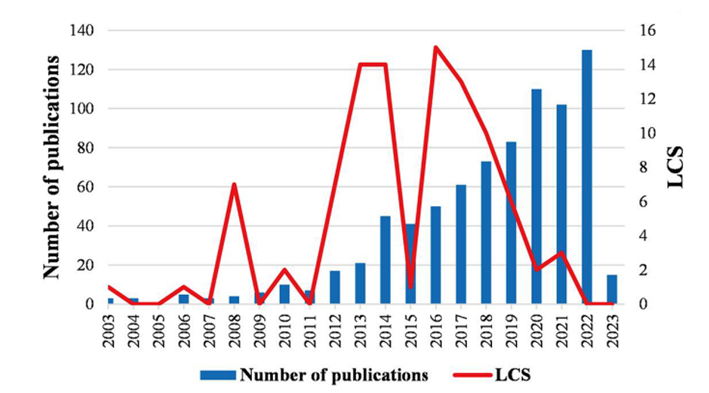
\includegraphics[width=\textwidth]{2/figures/Tendencia.png}
	\caption{Número de publicaciones relacionadas con mHealth. Fuente: \cite{global_trends_mhealth_2023}}
	\label{7:fig}
\end{figure}

Como se aprecia en la Figura N°\ref{7:fig}, el número de publicaciones relacionadas con mHealth ha ido en aumento, especialmente a partir de 2007, mostrando un crecimiento sostenido de más de 100 artículos por año desde 2020. Este incremento se debe, en gran medida, al impulso de la tecnología móvil y el impacto de la pandemia de COVID-19, que aceleró el desarrollo de herramientas de aprendizaje remoto y de salud digital en el ámbito educativo. En los últimos cinco años, la investigación en este campo ha experimentado un auge, con alrededor de 130 artículos nuevos publicados anualmente.
En los siguientes párrafos se detallan los estudios clave sobre mHealth en educación médica, los cuales servirán de base para el planteamiento de teorías y estrategias en el ámbito de la salud digital que se abordarán en este capítulo.


Un primer trabajo corresponde a \parencite{pascucci2021}, donde se desarrolló una aplicación móvil basada en inteligencia artificial (IA) con el objetivo de realizar análisis de resistencia antimicrobiana mediante pruebas de susceptibilidad a antibióticos (AST) en entornos con recursos limitados. La aplicación permite capturar imágenes de antibiogramas usando la cámara de un smartphone y, mediante algoritmos de procesamiento de imágenes y aprendizaje automático, analiza automáticamente las zonas de inhibición alrededor de los discos de antibióticos, proporcionando una interpretación de los resultados.
El objetivo principal fue desarrollar una herramienta móvil accesible y autónoma para realizar análisis de resistencia a antibióticos en entornos con recursos limitados, donde los sistemas de prueba automáticos suelen ser costosos o no están disponibles. La metodología incluyó el uso de algoritmos avanzados para el procesamiento de imágenes, basados en una biblioteca desarrollada en C++ que utiliza OpenCV y TensorFlow. Estos algoritmos permiten detectar y medir las zonas de inhibición en los antibiogramas, identificando los discos de antibióticos y ajustándose a los estándares de clasificación de susceptibilidad. Además, la aplicación cuenta con un sistema experto que evalúa la coherencia de los resultados de los AST, utilizando reglas de interpretación de comités internacionales como el EUCAST (European Committee on Antimicrobial Susceptibility Testing). Este sistema permite interpretar los resultados de manera automatizada, proporcionando diagnósticos y alertas de resistencia.
Para evaluar el rendimiento de la aplicación, se realizaron pruebas con tres conjuntos de datos de antibiogramas. Dos de estos conjuntos (A1 y A2) provenían de un hospital universitario en Créteil, Francia, y consistían en 570 y 75 muestras, respectivamente, procesadas durante la rutina diaria de laboratorio. El tercer conjunto (A3) se generó en un hospital de Médicos Sin Fronteras en Ammán, Jordania, utilizando microorganismos estandarizados de la American Type Culture Collection (ATCC). La precisión de la aplicación se comparó con la lectura manual (considerada estándar de oro) y con sistemas automáticos comerciales. La aplicación mostró una precisión del 90\% en la categorización de susceptibilidad frente a un sistema hospitalario automático y un 98\% en comparación con la medición manual, reduciendo la variabilidad entre operadores. Podemos apreciar mejor estos resultados en la Figura N°\ref{8:fig}

\begin{figure}[ht]
	\centering
	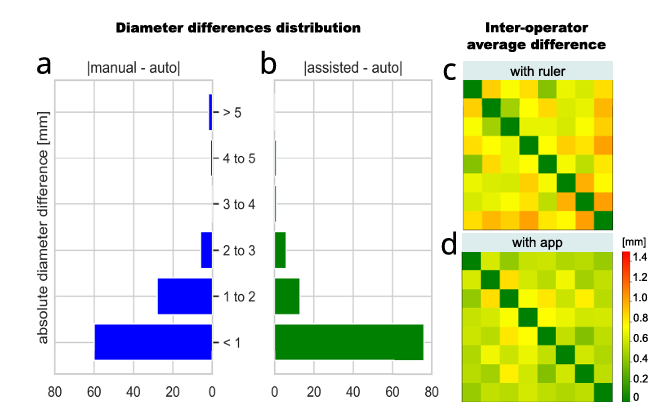
\includegraphics[width=\textwidth]{2/figures/R1.png}
	\caption{Resultados de referencia en el conjunto de datos A3. Los histogramas (a,b) muestran la distribución de las diferencias absolutas de diámetro entre el procedimiento automático de la App (auto) y la medición manual con regla (a), así como con el diámetro ajustado en el teléfono inteligente por los técnicos (asistido, b). A la derecha, los mapas de calor muestran la diferencia de medición absoluta promedio entre los ocho técnicos (dados dos lectores i y j, el cuadrado i, j representa la diferencia promedio entre ellos) que miden con la regla (c) y en modo asistido con la App (d). La medición asistida parece reducir la variabilidad entre operadores.. Fuente: \cite{pascucci2021}}
	\label{8:fig}
\end{figure}

La aplicación emplea estos conjuntos de datos como base de referencia para evaluar y optimizar sus algoritmos de medición de diámetros de inhibición y su sistema de interpretación. Además, el sistema experto contiene una base de conocimiento integrada, actualizada regularmente, que permite interpretar los resultados en función de las reglas de susceptibilidad del EUCAST. Gracias a su diseño offline y su compatibilidad con smartphones básicos, la aplicación resulta adecuada para su uso en áreas con recursos limitados, ampliando el acceso a pruebas de susceptibilidad y apoyando la lucha contra la resistencia antimicrobiana a nivel global.
 
Un segundo trabajo corresponde a \parencite{leung2022}, en el cual se desarrolló un sistema de recomendación basado en procesamiento de lenguaje natural (PLN) para identificar pacientes con cáncer que experimentan desafíos psicosociales y proporcionarles apoyo en el autocuidado a través de grupos de apoyo en línea. El objetivo principal fue implementar un sistema que detecte preocupaciones psicosociales en tiempo real durante las sesiones de grupo y recomiende recursos en línea personalizados para cada paciente, facilitando así el acceso a apoyo sin añadir carga adicional para los terapeutas.
La metodología incluyó el desarrollo de un algoritmo de PLN entrenado con un corpus de aproximadamente 80,000 mensajes de sesiones de apoyo en línea de CancerChatCanada (CCC). Se empleó el modelo Word2Vec para representar palabras en un espacio vectorial, permitiendo identificar expresiones semánticamente similares y extraer preocupaciones de los pacientes. Posteriormente, un sistema de recomendación asignó los recursos más adecuados según el perfil del paciente, tomando en cuenta factores como tipo de cáncer, edad, nivel de participación, síntomas de depresión y ansiedad, y estatus de cuidador. La base de datos de recursos consistió en 37 recursos en línea curados por terapeutas de CCC, evaluados en cuanto a su accesibilidad, relevancia y calidad.
\begin{figure}[ht]
	\centering
	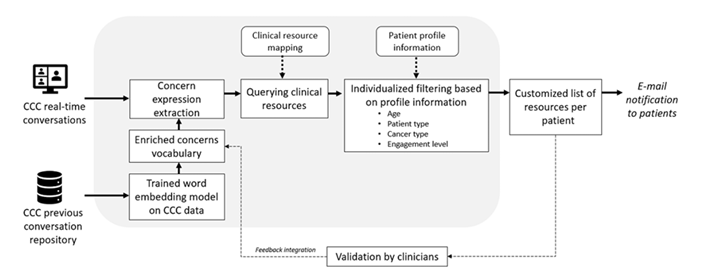
\includegraphics[width=\textwidth]{2/figures/CANADA.png}
	\caption{Descripción general del marco del sistema de recomendación de cofacilitadores basado en inteligencia artificial. CCC: CancerChatCanada. Fuente: \cite{leung2022}}
	\label{9:fig}
\end{figure}

Los resultados del sistema mostraron una alta precisión y capacidad de recuperación. Tras tres rondas de evaluación y mejora, el sistema alcanzó una precisión de 79.7\%, una recuperación de 98.1\% y una puntuación F1 de 88.0\%. De los 48 pacientes a quienes se les recomendaron recursos, el 52\% accedió a al menos un recurso, y el 76\% de estos pacientes encontró los recursos útiles. Estos hallazgos sugieren que el sistema basado en PLN es efectivo para ofrecer apoyo psicosocial personalizado a pacientes de cáncer en grupos de apoyo en línea, aumentando la accesibilidad a recursos relevantes y mejorando la experiencia del paciente en el manejo de sus desafíos emocionales y psicosociales.

Un tercer trabajo corresponde a \parencite{lee2024}, quienes desarrollaron un chatbot de atención médica basado en ChatGPT para proporcionar respuestas médicas precisas a pacientes con cáncer. El objetivo principal de este trabajo fue crear un servicio de chatbot que, mediante modelos de lenguaje natural (LLM), pueda brindar información médica confiable y específica para pacientes oncológicos en tiempo real, abordando las necesidades de información no satisfechas de estos pacientes.
La metodología en la figura N°\ref{9:fig} incluyó la creación de una base de datos especializada en conocimientos médicos sobre cáncer, construida con la colaboración de expertos en oncología. La base de datos integró guías prácticas acreditadas de distintas asociaciones médicas, incluyendo la Red Nacional de Cáncer de los Estados Unidos y la Sociedad Europea de Oncología, resultando en un meta-dataset de 1.17 millones de tokens. Este dataset fue categorizado en áreas como definición, epidemiología, causas, síntomas, diagnóstico, y tratamiento. La implementación del chatbot se realizó utilizando Python, combinando la API de OpenAI y el framework LangChain para facilitar la escalabilidad y permitir interacciones en múltiples idiomas.

\begin{figure}[ht]
	\centering
	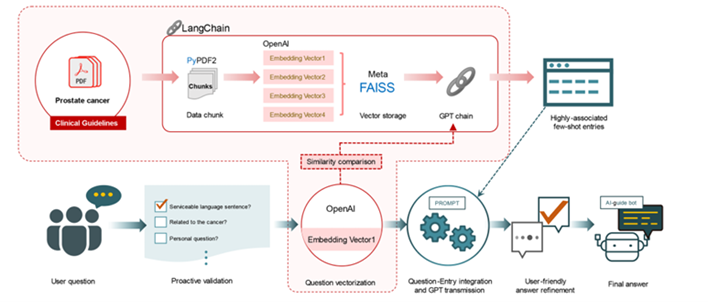
\includegraphics[width=\textwidth]{2/figures/BOT IA.png}
	\caption{Proceso de desarrollo de un bot basado en inteligencia artificial para pacientes con cáncer Fuente: \cite{lee2024}}
	\label{9:fig}
\end{figure}
Para la evaluación del rendimiento, el chatbot fue probado con un conjunto de 100 preguntas relacionadas con el cáncer, seleccionadas y validadas por oncólogos para garantizar respuestas precisas y actualizadas. La precisión, claridad y facilidad de lectura de las respuestas fueron evaluadas usando una escala Likert, donde se obtuvo un puntaje total promedio de 90.98. Estos resultados muestran que el chatbot fue efectivo en comprender las preguntas y en proporcionar respuestas claras y precisas, contribuyendo así a mejorar la accesibilidad de los pacientes a información médica verificada y a reducir la dependencia de fuentes poco confiables en internet.

Un cuarto trabajo corresponde a \parencite{smak2023}, en el cual se desarrolló un estudio piloto de viabilidad para evaluar el uso de una aplicación móvil basada en inteligencia artificial (IA) llamada SkinVision para el diagnóstico de cáncer de piel en el hogar. El objetivo principal de este estudio fue investigar las condiciones y la viabilidad de implementar una aplicación de salud móvil en la atención primaria para detectar lesiones cutáneas sospechosas, facilitando así la atención inicial y reduciendo las consultas innecesarias con médicos generales.
La metodología utilizada fue un diseño de métodos mixtos con la participación de tres prácticas de médicos generales en los Países Bajos. Durante el estudio, se incluyeron 50 pacientes que utilizaron la aplicación para evaluar sus lesiones cutáneas antes de consultar a su médico. La aplicación emplea una red neuronal convolucional para clasificar las fotos de las lesiones cutáneas como de alto o bajo riesgo, sugiriendo a los usuarios de alto riesgo que visiten a su médico. Además, los datos cualitativos fueron recolectados mediante observaciones, diarios de audio y entrevistas con los pacientes y médicos para comprender mejor las experiencias y percepciones del uso de la aplicación.
Los resultados mostraron una tasa de éxito del 84\% en la participación de los pacientes y del 90\% en la de los médicos generales. De los pacientes con lesiones benignas y clasificación de bajo riesgo, el 54\% indicó que se sentiría seguro cancelando su cita con el médico. Aunque la precisión de la aplicación fue alta, no cambió significativamente la precisión diagnóstica de los médicos, aunque en algunos casos influyó en el plan de tratamiento.
Este estudio no menciona una base de datos específica para entrenamiento o evaluación de la aplicación, ya que SkinVision es una aplicación validada y registrada en Europa. Los hallazgos preliminares sugieren que es factible implementar una aplicación basada en IA para la detección de cáncer de piel en entornos de atención primaria, lo que podría reducir la carga en los médicos generales al disminuir las consultas para lesiones benignas.

Un quinto trabajo corresponde a \parencite{jagadish2024}, en el cual se desarrolló una aplicación móvil basada en inteligencia artificial (IA) para ayudar a personas con discapacidad visual. El objetivo principal de esta aplicación fue mejorar la accesibilidad y promover la independencia de las personas con discapacidades visuales, brindándoles información en tiempo real sobre su entorno y facilitando actividades cotidianas.
La metodología incluyó la selección y entrenamiento de algoritmos de IA específicos para cada función de la aplicación, como reconocimiento de objetos, reconocimiento de color, lectura de texto y detección de billetes. Para entrenar estos modelos se utilizaron conjuntos de datos relevantes, como imágenes de objetos y colores, datos de texto para lectura de billetes y códigos de barras, y modelos preentrenados en TensorFlow Lite. La aplicación se desarrolló para funcionar en dispositivos Android, integrando características como comandos de voz, modos de alto contraste y compatibilidad con lectores de pantalla para garantizar la accesibilidad.
Los resultados demostraron que la aplicación puede reconocer y describir objetos, identificar colores en tiempo real, leer texto en voz alta y detectar billetes, ofreciendo así una experiencia más autónoma y segura para los usuarios con discapacidad visual. La interfaz fue diseñada para ser intuitiva y accesible, con retroalimentación táctil y compatibilidad con comandos de voz. El sistema funciona de manera offline, lo que permite su uso en áreas con conectividad limitada.
Este trabajo no menciona una base de datos específica para almacenar datos de los usuarios o resultados de detección; sin embargo, utiliza conjuntos de datos de entrenamiento y modelos preentrenados para lograr la funcionalidad de reconocimiento y descripción en tiempo real. Este proyecto resalta el potencial de las aplicaciones móviles basadas en IA para mejorar la accesibilidad y calidad de vida de personas con discapacidades visuales.

Un sexto trabajo corresponde a \parencite{khan2020}, quienes realizaron una revisión sistemática sobre la aplicación de inteligencia artificial (IA) y análisis de big data en el ámbito de la salud móvil (m-health), con el objetivo de identificar cómo estas tecnologías pueden mejorar los sistemas de atención médica. Este estudio tuvo como objetivo principal evaluar las aplicaciones actuales de IA y big data en m-health y proponer un modelo que optimice el uso de estas tecnologías para enfrentar desafíos específicos en la salud móvil.

La metodología empleada consistió en una revisión sistemática de artículos científicos, recopilando 106 estudios relevantes de bases de datos como IEEE Xplore, ACM Digital Library y ScienceDirect. Los artículos seleccionados abordan aplicaciones de IA y big data en salud móvil, utilizando criterios de inclusión y exclusión basados en el uso de estas tecnologías en el monitoreo de salud, diagnóstico y análisis de datos médicos. Se utilizó el diagrama de flujo Prisma como se ve en la figura N°\ref{10:fig} para el proceso de revisión.

\begin{figure}[H]
	\centering
	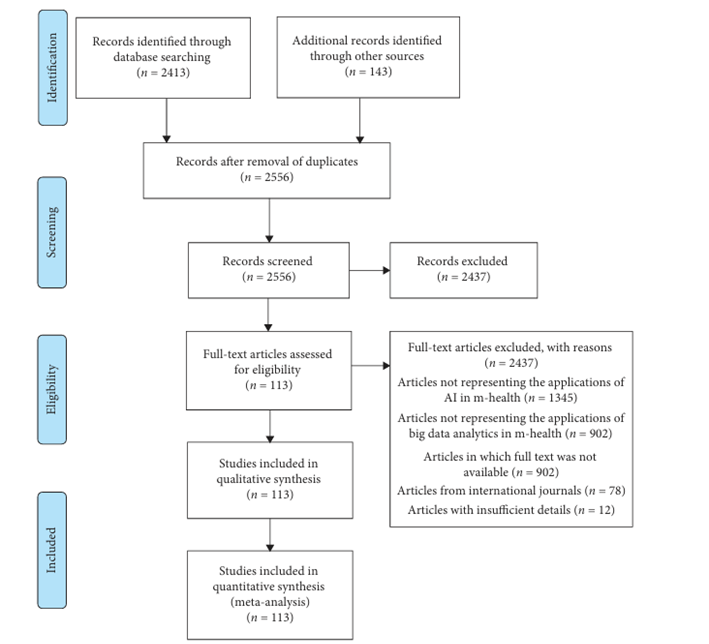
\includegraphics[width=\textwidth]{2/figures/PRISMA.png}
	\caption{Diagrama de Flujo Prisma para el proceso de revisión de artículos. Fuente: \cite{khan2020}}
	\label{10:fig}
\end{figure}



Los resultados de esta revisión destacaron aplicaciones de IA para el análisis de datos de salud, como el uso de sensores móviles para monitorear condiciones físicas y mentales, así como la implementación de modelos de aprendizaje automático para mejorar la precisión en el diagnóstico. Se propuso un modelo basado en IA y big data para m-health (ver figura N°\ref{11:fig}), que incluye la recolección de datos mediante dispositivos móviles, el análisis de big data, y una plataforma para la toma de decisiones en tiempo real.

\begin{figure}[H]
	\centering
	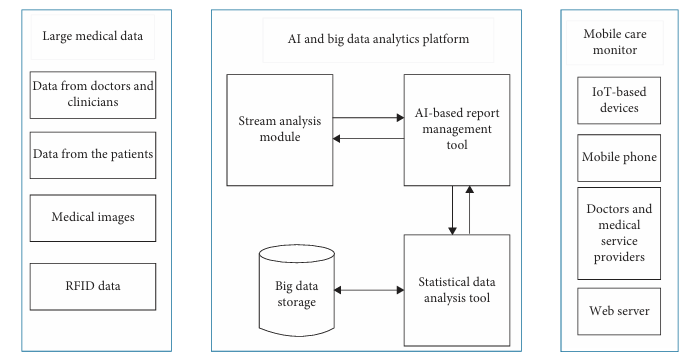
\includegraphics[width=\textwidth]{2/figures/MODELO.png}
	\caption{Modelo basado en IA y big data para m-health. Fuente: \cite{khan2020}}
	\label{11:fig}
\end{figure}

\vspace{0.5 cm}
Este estudio no emplea una base de datos específica, pero sugiere el uso de grandes volúmenes de datos médicos provenientes de registros electrónicos de salud (EHRs), imágenes médicas y otros datos clínicos para optimizar el m-health. Los hallazgos subrayan el potencial de la IA y el big data para mejorar la calidad de los sistemas de m-health, facilitando el acceso a información en tiempo real y mejorando la toma de decisiones clínicas.







Un séptimo  trabajo corresponde a \parencite{prevljak2024}, en el cual se exploró la aplicación de inteligencia artificial (IA) en la detección de cáncer de mama y en el monitoreo de resultados de laboratorio. El objetivo principal de este estudio fue mejorar la precisión y velocidad en el diagnóstico temprano del cáncer de mama, utilizando IA para analizar imágenes médicas y biomarcadores, lo cual contribuiría a una detección temprana y a reducir la tasa de resultados falsos negativos.
La metodología incluyó una revisión exhaustiva de 60 artículos científicos sobre la implementación de IA en la investigación del cáncer de mama, con datos recopilados de bases de datos como PubMed. El estudio analizó técnicas de aprendizaje profundo, especialmente redes neuronales convolucionales (CNN), aplicadas en el procesamiento de imágenes de mamografía, MRI y PET-CT, así como el análisis de biomarcadores. Los algoritmos de IA fueron entrenados para identificar patrones sutiles y anormalidades en imágenes médicas, ayudando a los profesionales en la toma de decisiones clínicas.
Los resultados del estudio indicaron que el uso de CNN y otras técnicas de IA en el análisis de imágenes aumentó significativamente la precisión en la detección de cáncer de mama en etapas tempranas. La IA también permitió la evaluación de biomarcadores como HER2 y Ki-67, mejorando la capacidad de personalizar los tratamientos según las características individuales del paciente. Estos hallazgos subrayan el potencial de la IA para transformar el diagnóstico y tratamiento del cáncer de mama, optimizando la toma de decisiones y mejorando los resultados en pacientes.


Un octavo antecedente corresponde al desarrollo de MentalApp, una aplicación móvil creada para facilitar el seguimiento del bienestar mental mediante herramientas personalizadas, tales como encuestas, sensores y comunicación directa con profesionales de la salud. Este proyecto fue llevado a cabo por un equipo de estudiantes de la Pontificia Universidad Javeriana y su propósito principal es brindar soporte a los usuarios en la gestión de su salud mental de una forma accesible y eficiente. La meta del proyecto fue migrar una plataforma web de salud mental a una aplicación móvil, con el fin de mejorar la accesibilidad y usabilidad para los usuarios jóvenes, ofreciendo un seguimiento y monitoreo más exhaustivo de su bienestar mental. 
La aplicación busca registrar y evaluar aspectos como el estado emocional, el estrés, el sueño y otros indicadores de salud mental, brindando recursos personalizados y acceso a profesionales de la salud. (Propuesta de solución Figura N°\ref{12:fig})

\begin{figure}[ht]
	\centering
	\includegraphics[width=\textwidth]{2/figures/PROPUESTA DE SOLUCIÓN.png}
	\caption{Propuesta de solución. Fuente: \cite{coral2023}}
	\label{12:fig}
\end{figure}

Para el desarrollo de MentalApp, se utilizó un enfoque de metodologías ágiles, combinando Scrum y Sawtooth. Esta elección metodológica permitió dividir las tareas en sprints con retroalimentación constante de los interesados. La estructura de la aplicación se fundamentó en una arquitectura en capas (Layered Pattern), que organiza la lógica de negocios, la integración, la presentación y el modelo de dominio. En cuanto a las herramientas utilizadas, el equipo empleó Flutter para el desarrollo de la interfaz, Java y Spring Boot para los servicios de backend, y MySQL como sistema de gestión de bases de datos. Además, se integró Jitsi Meet para permitir videollamadas. La aplicación incluyó también el uso de sensores mediante la integración de la API de reconocimiento de actividad (Activity Recognition API) de Android para monitorear actividades físicas de los usuarios. Sin embargo, debido a las políticas de Google Play Store, la recopilación de datos del GPS se limitó a situaciones en las que la aplicación se ejecutaba en primer plano. Para asegurar el correcto funcionamiento del sistema antes de la versión Alpha, se realizaron pruebas de componentes y evaluaciones en sprints. Asimismo, se llevaron a cabo encuestas de satisfacción con usuarios para evaluar la facilidad de uso y la utilidad de la aplicación. La implementación de todo esto se puede apreciar en la figura N°\ref{13:fig}

\begin{figure}[ht]
	\centering
	\includegraphics[width=\textwidth]{2/figures/IMPLEMENTACIÓN MENTALAPP.png}
	\caption{Implementación MentalAPP. Fuente: \cite{coral2023}}
	\label{13:fig}
\end{figure}

Entre los componentes principales de MentalApp, se encuentran las encuestas periódicas, que permiten a los usuarios completar evaluaciones sobre distintos aspectos de su salud mental, como el estrés, el sueño y el bienestar emocional. La aplicación también incluye un plan de bienestar que permite a los usuarios registrar actividades, crear contactos de emergencia y gestionar signos de alarma, ofreciendo un seguimiento personalizado de su estado de salud mental. Otra funcionalidad importante es la comunicación directa con profesionales de la salud, donde los usuarios pueden solicitar orientación mediante chat o videollamadas, accediendo así a apoyo psicológico en tiempo real. Además, MentalApp ofrece recursos personalizados a los usuarios, como artículos y recomendaciones específicas de acuerdo con sus necesidades, propuestas por profesionales de la salud.
Las pruebas de usuario revelaron que los participantes encontraron la aplicación fácil de entender, intuitiva y satisfactoria en términos de experiencia de usuario. Estos resultados también indicaron una alta probabilidad de recomendación de la aplicación, lo que sugiere un impacto positivo en su aceptación general. MentalApp utiliza tres bases de datos relacionales en MySQL, cada una con un propósito específico: RegisterDB, que contiene los datos de los usuarios, incluyendo su historial médico y registros de orientación; SurveyDB, que almacena los resultados de las encuestas y los datos obtenidos de los sensores; y BotnarDB, que gestiona los planes de bienestar y las relaciones entre los usuarios y los profesionales de la salud. Este antecedente demuestra cómo una aplicación móvil puede ser una herramienta eficaz en el monitoreo y apoyo a la salud mental, especialmente en poblaciones jóvenes que enfrentan barreras de acceso a servicios de salud mental. MentalApp facilita el seguimiento de indicadores clave de bienestar y permite a los usuarios recibir recomendaciones personalizadas y apoyo profesional de manera accesible y conveniente.
